\title{Report on \\ Model Development for Fossil Fuel Divestment}
\author{Jakob J. Kolb \\ Potsdam Institute for Climate Impact Research}

\maketitle

\section{Model Development}

Previous studies \cite{Ans2013} suggest that feedback through supply-demand price mechanisms will have only limited impact on fossil fuel companies. This is due to the fact, that only approximately 15 \% of investors invest subject to socially responsible guidelines \cite{SIF2014Report} and that divested holdings are, especially in liquid markets, very likely to quickly find their way to less responsible investors. \\
Therefore, the effects of a divestment campaigns on target industries rather stem from `soft' factors such as changes in market norms and stigmatization and growing uncertainty about future business opportunities. This means that for the understanding of the campaign dynamics, opinion spreading with respect to beliefs about future business development and respective uncertainties amongst investors might be worth a closer look. \\
In the following I propose a preliminary scheme of such a model.

\begin{figure}[h]
	\centering
	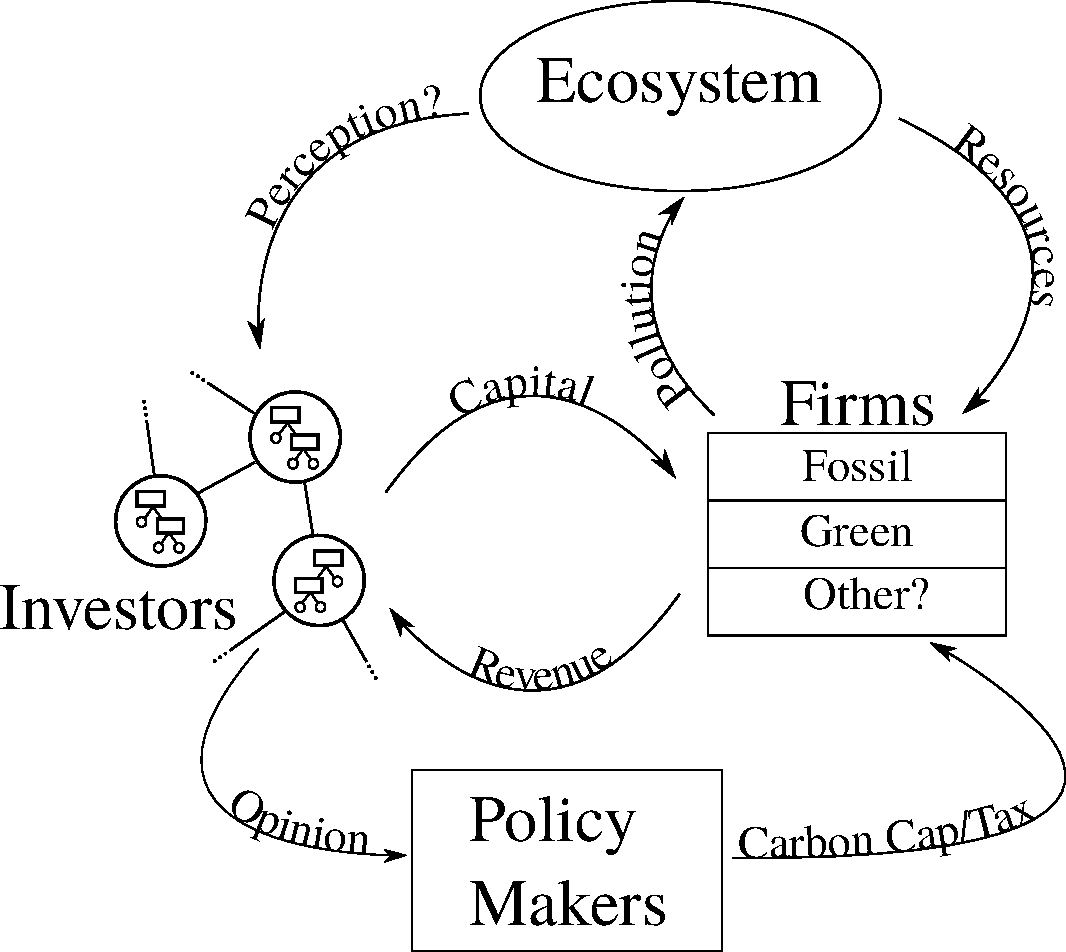
\includegraphics[width = .7 \textwidth]{Model_Scheme.pdf}
	\caption{Schematic sketch of the model including four major components: Households, Firms (grouped by sector), Ecosystem and optional Policy makers.}
	\label{fig:model}
\end{figure}

\subsection{Ramsey-Cass-Koopmans Model of optimal saving}


\subsection{Sectors}

Production is assumed to take place in two sectors. One sector $(d)$ employs a dirty technology depending on fossil resources, the other sector $(c)$ employs a clean technology relying on renewable resources. The physical capital is assumed to be bound to this technology, e.g. there are two separate capital stocks $K_d$ and $K_c$. Both sectors use capital $K_j$ and labor $P_j$ as input factors, the dirty sector additionally uses a fossil resource $R$.
\begin{equation}
	Y_j = F_j(K_j,P_j,R), \qquad \frac{\partial Y_c}{\partial R} = 0 	
	\label{eq:production}
\end{equation}
The total cost for fossil resource extraction $c_R$ (exploration and exploitation) is assumed to scale with $R^{\varepsilon}$.
\begin{equation}
	c_R = b_R R_d^{\varepsilon}
	\label{resource_extraction_cost}
\end{equation}
The factor $b_R$ is presumably depending on the remaining Fossil resource $G$ and increasing as the remaining resource decreases. It is assumed to diverge, as $G$ approaches zero. Also, for optimal production, resource uptake is adjusted such that the marginal extraction costs are equal to the marginal productivity of the resource:
\begin{equation}
	b_R \varepsilon R_{d}^{\varepsilon-1} = \frac{\partial F_d}{\partial R_d}
	\label{marginal_resource_extraction_cost}
\end{equation}
For high [low] intensity of fossil resource use, i.e. $R \gg 1$ [$R \ll 1$], productivities of other input factors are assumed to be higher [lower] in the dirty sector compared to the clean sector:
\begin{align}
	R \gg 1 \quad \Rightarrow & \quad \frac{\partial Y_d}{\partial K_d} > \frac{\partial Y_c}{ \partial K_c}, \quad \frac{\partial Y_d}{\partial P} > \frac{\partial Y_c}{ \partial P}, \\
	R \ll 1 \quad \Rightarrow & \quad \frac{\partial Y_d}{\partial K_d} < \frac{\partial Y_c}{ \partial K_c}, \quad \frac{\partial Y_d}{\partial P} < \frac{\partial Y_c}{ \partial P}.
	\label{eq:input_factor_productivities}
\end{align}
For the input factor markets, market clearing is assumed. Capital rental rate and wages are thereby determined by marginal factor productivities of the respective input factors.
For wages, this results in the following conditions:
\begin{equation}
	\left. \frac{\partial Y_d}{ \partial P} \right|_{P_d} = \left. \frac{\partial Y_c}{\partial P}\right|_{P_c} = w, \qquad P_d + P_c = \sum_i P_i
	\label{eq:wage_rage}
\end{equation}
and for the capital rental rate this results in the following conditions:
\begin{align}
	\left. \frac{\partial Y_d}{\partial K}\right|_{K_d} &= r_d,\quad K_d = \sum_i K^{(d)}_i \nonumber \\
	\left. \frac{\partial Y_c}{\partial K}\right|_{K_c} &= r_c,\quad K_c = \sum_i K^{(c)}_i 
	\label{eq:capital_rental_rate}
\end{align}


\subsection{Households}

\textbf{Income and savings accounting:} \\
Households denoted with the Index $i$, $i \in [1, \dots N]$ are are owners of capital $K_j$ as well as suppliers of labor $P_j$. A household has $P_i$ members, each supplying one unit of labor per unit of time $t$. The income of the household comes from capital returns and labor income:
\begin{equation}
	I_i = \sum_j r_j K^{(j)}_{i} + wP_i 
	\label{eq:household_income}
\end{equation}
Households are assumed to save at a fixed rate $s$ and reinvest their savings in one of the two types of capital ($K_c$ and $K_d$) available.
\textit{ For now, capital investment is considered irretrievable and capital can not be traded. Empirical data suggests a more or less constant savings rate of 23 \%} \\

\textbf{Savings investment - decision making:} \\
Households have to decide in which of the two capital goods they want to invest their savings. This decision processes is assumed to be bounded rational and are implemented in the framework of Fast and Frugal Heuristics.\\
Decision cues are:
\begin{table}[H]
	\centering
	\begin{tabular}{ll}
		$ROI = \frac{r_j(t)}{\delta_j}$ & total return of investment over lifetime according to current return rate,\\
		$DR = E_{t-\Delta t, t}[\dot{r}_j]$ & Dynamics of rate of return in sector $j$ during previous investment period, \\
		$MORAL$ & Whether the investment is clean or dirty, \\
		$GROUP$ & majority vote amongst neighbors. \\
	\end{tabular}
	\caption{Definition of investment decision cues}
	\label{tab:decision_cues}
\end{table}

\textit{Open questions}
\begin{itemize}
	\item Exact definition of decision problem e.g. binary choice? satisficing and accept/reject with fast and frugal tree?
\end{itemize}

\textbf{Opinion formation and social dynamics:} \\
The structure $S$ of the decision heuristics is interpreted as preferences/opinions resulting from conceptual social dynamic. \\
Technically, this means that households are connected by a social network. Households are nodes, connections are links, links form an unweighted, undirected network that is represented by an adjacency matrix $A_{kl}$.
The dynamics of and on the network is the following:
The activity of households is given by a Poisson process e.g. the times $\Delta t$ after which a household becomes active are distributed as
\begin{equation}
	p(\Delta t) = \frac{1}{\tau} \rm{exp}\left[-\frac{\Delta t}{\tau} \right].
	\label{waiting_time_distribution}
\end{equation}
If it becomes active, it does the following:
\begin{itemize}
	\item it chooses one of his neighbors to compare itself to,
	\item if their preferences differ, one of two things happen:
	\item with probability $\varphi$ the selected household $k$ cuts
		the link to the selected neighbor $l$ and establishes a new
		link to a random neighbor with the same preferences
	\item with probability $1-\varphi$ they compare a fitness parameter $W_k$
		which is household income in our case: 

		\begin{equation}
			W_i = \sum_j r_j K^{(j)}_{i} + wP_i.
			\label{eq:fitness}
		\end{equation}

		if if the neighbors fitness is higher, the active household $k$
		adopts the neighbor $k$'s preferences $(S_k \rightarrow S_l)$ with a sigmoid shaped 
		probability:
		\begin{equation}
			P(S_k \rightarrow S_j) = 1/2 (\rm{tanh}(W_k - W_l)-1)
			\label{imitation_probability}
		\end{equation}
\end{itemize}

\subsection{Ecosystem}
Ecosystem is the source of resources and the sink for pollution. Minimal implementation would be a fixed carbon stock that is exploited by the fossil fuel sector. Optionally one could implement some sort of climate impact as a consequence of pollution.

In the case under study, we assume a non renewable geological carbon stock $G$, that is exploited by fossil resource uptake of the dirty sector:
\begin{equation}
	\dot{G} = -R
	\label{resource_dynamics}
\end{equation}

\subsection{Policy Makers}
\textit{Optional:} \\
Policy makers can implement some carbon tax or carbon cap on economy to incentivize green development. The implementation of such measure depends on the prevalence of opinions amongst voters (are investors a representative sample of voters?) and might be appropriately implemented by a Poisson distributed random variable.

\subsection{Variables}

\subsubsection{Independent variables:}

\begin{table}[H]
	\centering
	\begin{tabular}{r|l}
		Variable & Description \\\hline
		$K^{(c)}_i(t)$ & clean investment of household $i$ \\
		$K^{(d)}_i(t)$ & dirty investment of household $i$ \\
		$P_i(t)$ & Members of household, $i$ \\
		$G(t)$ & Geological carbon stock \\
		$A_{kl}(t)$ & Adjacency matrix \\
		$x_i(t) \in [c,d]$ & investment decision of household $i$ 
	\end{tabular}
	\caption{Variables of the model with description.}
	\label{tab:independent_variables}
\end{table}

\subsubsection{Derived Variables}

\begin{table}[H]
	\centering
	\begin{tabular}{r|l}
		Variable & Description \\\hline
		$w(t)$   & Wage rate, \\
		$r_j(t)$ & Capital return rate in sector $j$, \\
		$c_R(t)$ & Fossil resource extraction cost, \\
		$Y_j(t)$ & Output of sector, $j$ \\
		$P_j(t)$ & total labor employed in sector $j$, \\
		$K_j(t)$ & Total capital employed in sector $j$, \\
		$R(t)$ & Rate of resource uptake of dirty sector. \\
	\end{tabular}
	\caption{Variables of the model with description.}
	\label{tab:derived_variables}
\end{table}

\subsection{Parameters}

\begin{table}[H]
	\centering
	\begin{tabular}{r|l}
		Parameter & Description \\\hline
		$\kappa_j$ & Capital elasticity in sector $j$ \\
		$\pi_j$ & Labor elasticity in sector $j$ \\
		$\rho$ & Fossil resource elasticity in dirty sector \\
		$b_j$ & total factor productivity in sector $j$ \\
		$b_R$ & resource uptake efficiency for fossil resource \\
		$s$ & savings rate \\
		$\delta $ & Capital depreciation rate \\
		$\tau$ & activity rate of households \\
		$\varphi$ & rewiring rate of households
	\end{tabular}
	\caption{Parameters of the model with description.}
	\label{tab:parameters}
\end{table}

\subsection{Dynamic equations}
To wrap up, the economic subsystem of the model can be described by the following ordinary differential equations:
\begin{align}
	\dot{K}_i^{(c)} &= s \delta(x_i - c) (r_c K_i^{(c)} + r_d K_i^{(d)} + w P_i) - \delta K_i^{(c)} \nonumber \\
	\dot{K}_i^{(d)} &= s \delta(x_i - d) (r_c K_i^{(c)} + r_d K_i^{(d)} + w P_i) - \delta K_i^{(d)} \nonumber \\
	\dot{P}_i &= \alpha P_i \nonumber \\
	\dot{G} &= - R 
\end{align}
that are subject to the following algebraic constraints:
\begin{align}
	P_c + P_d &= P \\
	\left. \frac{\partial Y_c}{\partial P} \right|_{P_c} &= \left. \frac{\partial Y_d}{\partial P} \right|_{P_d} \\
	\frac{\partial c_R}{\partial R} &= \frac{\partial Y_d}{\partial R} 
\end{align}
and $r_c$, $r_d$ and $w$ are given by the respective marginal productivities:
\begin{equation}
	r_c = \left. \frac{\partial Y_c}{\partial K} \right|_{K_c}, \qquad r_d = \left. \frac{\partial Y_d}{\partial K} \right|_{K_d}, \qquad w = \left. \frac{Y_c}{\partial P} \right|_{P_c} 
\end{equation} 


\section{Implementation}

Lets assume a Cobb Douglas production function:
\begin{equation}
	F_j(K_j,P_j,R_j,t) = b_j K_j^{\kappa_j}P_j^{\pi_j}R_j^{\rho_j}, \qquad j = c,d.
	\label{cobb_douglas}
\end{equation}
For the clean sector, $\rho_c = 0$ since it does not depend on the fossil resource. We assume equal labor elasticities in both sectors ($\pi_c = \pi_d$).

The general equilibrium solution for the input factors for the two sectors pose algebraic constraints for the system of ordinary differential equations that describe the dynamics of the capital stocks $\dot{K}_i^{(j)}$, the resource stock $\dot{G}$ and the population growth $\dot{P}_i$

\subsection{Market clearing for capital $K$:}

\begin{align}
	&K_c = \sum_i K_i^{(c)}, \quad r_c = b_c\kappa_c K_c^{\kappa_c-1} P_c^{\pi}, \\
	&K_d = \sum_i K_i^{(d)}, \quad r_d = b_d\kappa_d K_d^{\kappa_d-1} P_d^{\pi}R_d^{\rho}.
	\label{capital_market_clearing}
\end{align}

The capital shares of the two sectors are not subject to an equilibrium solution and can be evaluated independently. For the calculation of the capital rent $r$, the solutions to labor shares and optimal resource use are necessary.

\subsection{Market clearing for labor $P$:}
The total supply of labor $P$ is given by the sum of the members of all households. The total supply of labor is divided amongst sectors such that the marginal productivities of labor are equal:
\begin{equation}
	P_c + P_d = P = \sum_i P_i, \qquad w = b_c K_c^{\kappa_c}\pi_c P_c^{\pi_c-1}=  b_d K_d^{\kappa_d}\pi_d P_d^{\pi_d-1}R_d^{\rho_d} 
	\label{labour_market_clearing}
\end{equation}
Substituting $X_c^{\beta-1} = b_c K_c^{\kappa_c}$ and $X_d^{\pi-1} = b_d K_d^{\kappa_d}$ the labor shares $P_c$ and $P_d$ are equal to
\begin{align}
	P_c = P \frac{X_d R^{\frac{\rho}{\pi-1}}}{X_c + X_d R^{\frac{\rho}{\pi-1}}} \label{labor_share_Pc}  \\
	P_d = P \frac{X_c}{X_c + X_d R^{\frac{\rho}{\pi-1}}} \label{labor_share_Pd}	
\end{align}
and the corresponding wage is given by
\begin{equation}
	w = \pi \left[ P \frac{X_c X_d}{X_c R^{\frac{-\rho}{\pi-1}} + X_d} \right]^{\pi-1}
	\label{wage}
\end{equation}

These solutions still depend on the uptake of fossil resource $R$.

\subsection{Optimal Resource use $R$:}

From equation \eqref{resource_extraction_cost} follows that
\begin{equation}
	b_R \varepsilon R_d^{\varepsilon-1} = b_d K_d^{\kappa_d}P_d^{\pi}\rho R^{\rho-1}
	\label{optimal_resource_extraction_condition}
\end{equation}
and consequently, the resource use $R$ is equal to
\begin{equation}
	R = X_R P_d^{\frac{\pi}{\varepsilon-\rho}}
	\label{optimal_resource_extraction}
\end{equation}
where $X_R$ is given by
\begin{equation}
	X_R = \left( \frac{\rho b_d K_d^{\kappa_d}}{ \varepsilon b_R} \right)^{\frac{1}{\varepsilon-\rho}}
	\label{optimal_resource_XR}
\end{equation}

\subsection{Elimination of algebraic constraints}

To system is easier to handle, if the ordinary differential equations are not subject to algebraic constraints. \\
Therefore, it is necessary to decouple equations \eqref{labor_share_Pc}, \eqref{labor_share_Pd} and \eqref{optimal_resource_extraction}.
From \eqref{labor_share_Pc} and \eqref{optimal_resource_extraction} it follows that
\begin{align}
	P_d &= P\frac{X_c}{X_c + X_d X_R^{\frac{\rho}{\pi-1}}P_d^{\frac{\rho}{\pi-1}\frac{\pi}{\varepsilon-\rho}}} \\
	P X_c P_d^{-1} &= X_c + X_d X_R^{\frac{\rho}{\pi-1}}P_d^{\frac{\rho}{\pi-1}\frac{\pi}{\varepsilon-\rho}} \\
	0 &= X_d X_R^{\frac{\rho}{\pi-1}}P_d^{\frac{\rho}{\pi-1}\frac{\pi}{\varepsilon-\rho}+1} + X_c P_d - P X_c
\end{align}
To find a solution for $P_d$ the exponents $\pi$, $\rho$ and $\varepsilon$ need to satisfy either \\
A:
\begin{equation}
	\frac{\rho}{\pi-1}\frac{\pi}{\varepsilon-\rho} = 1
\end{equation}
or B:
\begin{equation}
	\frac{\rho}{\pi-1}\frac{\pi}{\varepsilon-\rho}= -1
\end{equation}
or C:
\begin{equation}
	\frac{\rho}{\pi-1}\frac{\pi}{\varepsilon-\rho}= 0
\end{equation}
For simplicity we assume case B which results in
\begin{align}
	\frac{\rho}{\pi-1}\frac{\pi}{\varepsilon-\rho} &= -1 \\
	\pi \rho &= -\pi\varepsilon + \pi\rho + \varepsilon - \rho \\
	\rho &= \varepsilon(1-\pi).
\end{align}
And thus $P_c$, $P_d$ and $R$ result in
\begin{align}
	P_c &= \frac{X_d }{X_c}X_R ^{-\varepsilon}, \\
	P_d &= P - \frac{X_d }{X_c}X_R ^{-\varepsilon}, \\
	R &= X_R \left( P-\frac{X_c}{X_d} X_R^{-\varepsilon} \right)^{\frac{1}{\varepsilon}}.
	\label{input_share_solution_IIb}
\end{align}
These results hold as long as $P_d>0$. Otherwise $P_c = P$, $P_d = 0$ and $R=0$. 

For $P_d>0$, $w$, $r_c$ and $r_d$ result in

\begin{align}
	w &= \pi X_d^{\pi-1} X_R ^{\rho}, \\
	r_c &= \frac{\kappa_c}{K_c X_c}X_d^{\pi}X_R^{-\varepsilon \pi}, \\
	r_d &= \frac{\kappa_d}{K_d}X_d^{\pi-1}X_R^{\rho}\left( P -\frac{X_d}{X_c}X_R^{-\varepsilon}\right).
\end{align}
Otherwise, 

With these results, we can rewrite the dynamical equations of the system:
\begin{align}
	\dot{K}_i^{(c)} = s \delta(x_i - c) \bigg(& C_4 \frac{K_c^{\kappa_c-1}}{G^2 K_d^{\kappa_d}} K_i^{(c)} \nonumber \\
	&+ C_5 \frac{K_c^{\kappa_c}}{G^2 K_d^{\kappa_d + 1}}\left( C_6 P (g^2 K_d^{\kappa_d})^{1/\pi} -1 \right) K_i^{(d)} \nonumber \\ 
	&+ C_3 K_c^{\kappa_c}(G^2K_d^{\kappa_d})^{\frac{1-\pi}{\pi}} P_i \bigg) - \delta K_i^{(c)} \\
	\dot{K}_i^{(d)} = s \delta(x_i - d) \bigg(& C_4 \frac{K_c^{\kappa_c-1}}{G^2 K_d^{\kappa_d}} K_i^{(c)} \nonumber \\
	&+ C_5 \frac{K_c^{\kappa_c}}{G^2 K_d^{\kappa_d + 1}}\left( C_6 P (g^2 K_d^{\kappa_d})^{1/\pi} -1 \right) K_i^{(d)} \nonumber \\ 
	&+ C_3 K_c^{\kappa_c}(G^2K_d^{\kappa_d})^{\frac{1-\pi}{\pi}} P_i \bigg) - \delta K_i^{(d)} \\
	\dot{P}_i &= \alpha P_i \nonumber \\
	\dot{G} &= - C_1(G^2 K_d^{\kappa_d})^{\frac{1}{\pi \varepsilon}}\left( P - C_2 \frac{K_c^{\frac{\kappa_c}{1-\pi}}}{G^{\frac{2}{\pi}}K_d^{\frac{\kappa_d}{(1-\pi)\pi}}} \right) 
\end{align}

For the analysis, we restrict the model to this second solution choosing 
\begin{equation}
	\pi = \frac{2}{5}, \qquad \rho = \frac{3}{4}, \qquad \varepsilon = \frac{5}{4}.
	\label{exponent_values}
\end{equation}

With $\kappa_c = \kappa_d = 3/5$ the equations that are finally encoded in the model are:

\begin{align}
	\dot{K}_i^{(c)} = s \delta(x_i - c) \bigg(&  r_c(K_c, K_d, G)  K_i^{(c)} \nonumber \\
	&+ r_d(K_c, K_d, G, P) K_i^{(d)} \nonumber \\ 
	&+w(K_c, K_d, G, P)  P_i \bigg) - \delta K_i^{(c)} \\
	\dot{K}_i^{(d)} = s \delta(x_i - d) \bigg(&  r_c(K_c, K_d, G)  K_i^{(c)} \nonumber \\
	&+ r_d(K_c, K_d, G, P) K_i^{(d)} \nonumber \\ 
	&+  w(K_c, K_d, G, P) P_i \bigg) - \delta K_i^{(d)} \\
	\dot{P}_i &= \alpha P_i \nonumber \\
	\dot{G} &= - R(K_c, K_d, G, P) 
\end{align}
with coupling functions:
\begin{align}
	R(K_c, K_d, G, P) &= C_1G^4 K_d^{6/5}\left( P - C_2 \frac{K_c}{G^5K_d^{5/2}} \right), \\
	w(K_c, K_d, G, P) &= C_3 G^3 K_c^{3/5}K_d^{9/10} , \\
	r_c(K_c, K_d, G) \quad &= \frac{C_4}{G^2 K_c^{2/5}K_d^{3/5}} , \\
	r_d(K_c, K_d, G, P) &= C_5 \frac{K_c^{3/5}}{G^2 K_d^{5/8}} \left( 1-C_6 G^5 K_d^{3/2} P \right) ,
	\label{final_rates_and_wages}
\end{align}
and parameters
\begin{align}
	C_1 &= to be written down..\nonumber \\
	C_2 &= \nonumber \\
	C_3 &= \nonumber \\
	C_4 &= \nonumber \\
	C_5 &= \nonumber \\
\end{align}

For first studies, the opinion formation part of the model is reduces to the trivial adaptive voter model as it is implemented in the Copan EXPLOIT model. When a household becomes active, it either rewires with probability $\varphi$, or imitates its neighbors investment decision (clean or dirty) with probability 

\begin{equation}
	P(x_k \rightarrow x_j) = 1/2 (\rm{tanh}(W_k - W_l)-1)
	\label{primitive_imitation_probability}
\end{equation}

With the fitness parameter equal to the households income.

\bibliography{PhD-Divestment.bib}{}
    \bibliographystyle{IEEEtran}
